\[
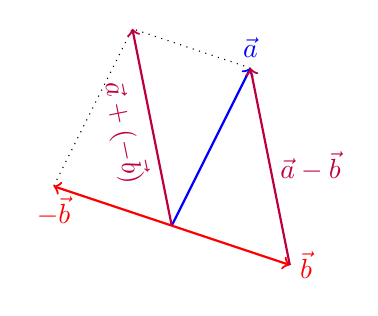
\begin{tikzpicture}[scale=1]
\coordinate (O) at (0,0);
\coordinate (A) at (1,2);
\coordinate (B) at (1.5,-0.5);
\coordinate (b) at (-1.5,0.5);
\coordinate (C) at (-0.5,2.5);
\pp
\draw[->,thick,blue](O)--(A) node[pos=1,above] {$\vec{a}$};
\draw[->,thick,red](O)--(B) node[pos=1,right] {$\vec{b}$};
\pp
\draw[->,thick,red](O)--(b) node[pos=1,below] {$-\vec{b}$};
\pp
\draw[dotted](A)--(C)--(b);
\pp
\draw[->,thick,purple](O)--(C) node[pos=0.5,sloped,below] {$\vec{a}+(-\vec{b})$};
\pp
\draw[->,thick,purple](B)--(A) node[pos=0.5,right] {$\vec{a}-\vec{b}$};
\end{tikzpicture}
\]